\begin{titlepage}
  \centering
  \vspace*{1cm}

  {\large Laboratorio No. 02 --- OS Setup, Shell y Software de Soporte de Red \par}
  \vspace{1.5cm}

  {\large Por: \par}
  {\large Camilo Aguirre \par}
  {\large Juan David Rangel \par}
  \vspace{1cm}

  {\large Profesor: John Alexander Pachón Pinzón \par}
  \vspace{1.5cm}

  {\large Escuela Colombiana de Ingeniería Julio Garavito \par}
  {\large Universidad \par}
  \vspace{0.5cm}

  {\large Arquitectura y Servicios de Red (AYSR) \par}
  \vspace{1.5cm}

  {\large Bogotá, D.C., viernes 21 de agosto de 2026 \par}

  \vfill
\end{titlepage}

\tableofcontents
\newpage

\section{Introducción}

Objetivo del laboratorio: familiarizarse con el software de soporte de red --- Packet Tracer y Wireshark ---, con la programación de scripts de shell, con el editor VI y con el despliegue de máquinas virtuales y compartición de archivos con SMB/SAMBA, sobre la plataforma de sistemas operativos montada en el Laboratorio 01.

Este informe es autosuficiente: toda la evidencia (capturas, comandos y salidas reales de ejecución) está incluida dentro del propio documento. Los videos de evidencia están publicados en YouTube y se enlazan en la sección correspondiente y en el Anexo A.

\section{Marco teórico}

\subsection{Packet Tracer}
Packet Tracer es un simulador de redes de Cisco que permite armar topologías, configurar dispositivos y observar el tráfico paquete por paquete en modo simulación. El curso introductorio de la plataforma (``Getting Started with Cisco Packet Tracer'') presenta los dispositivos de red, los modos de operación y el análisis de PDUs.

\subsection{Encapsulación}
Cada capa del modelo OSI/TCP-IP agrega su encabezado a los datos de la capa superior: los datos de aplicación se encapsulan en un mensaje ICMP/TCP, este en un paquete IP y este en una trama Ethernet. En el destino se desencapsula en orden inverso. Esto se observa tanto en Packet Tracer (PDUs) como en Wireshark (tráfico real).

\subsection{Wireshark}
Wireshark es un analizador de protocolos (sniffer) que captura los paquetes de una interfaz de red y los decodifica capa por capa. En modo promiscuo, la NIC captura todas las tramas del segmento, no solo las dirigidas a su propia MAC.

\subsection{SMB / SAMBA}
SMB (Server Message Block) es el protocolo de compartición de archivos e impresoras en redes Windows. SAMBA es la implementación libre que permite a sistemas Unix actuar como servidores o clientes SMB. Solaris 11.4 incluye un servidor SMB nativo gestionado por SMF y el paquete \texttt{service/network/samba} para el servicio clásico.

\subsection{Scripts de shell y editor VI}
El shell de Unix permite automatizar tareas de administración mediante scripts. VI es el editor de texto estándar de los sistemas Unix, con modos de operación (normal/inserción/comando).

\section{Desarrollo}

\subsection{1. Getting to Know Packet Tracer}

\textbf{Versión de Packet Tracer en la plataforma Cisco:} \texttt{9.0.1} (disponible en NetAcad).

\textbf{Video resumen del curso (capítulos 1--4, máx. 5 min):} participan los dos integrantes. Duración: 3:42.
\begin{itemize}
  \item Enlace: \href{https://youtu.be/RGuyiOb2aH4}{\url{https://youtu.be/RGuyiOb2aH4}}
\end{itemize}

\textbf{Quiz ``Introduction to Packet Tracer - PT Basics Quiz'' (individual):} cada integrante rindió el quiz y guardó captura del resultado (figura \ref{fig:quiz}).

\begin{figure}[H]
  \centering
  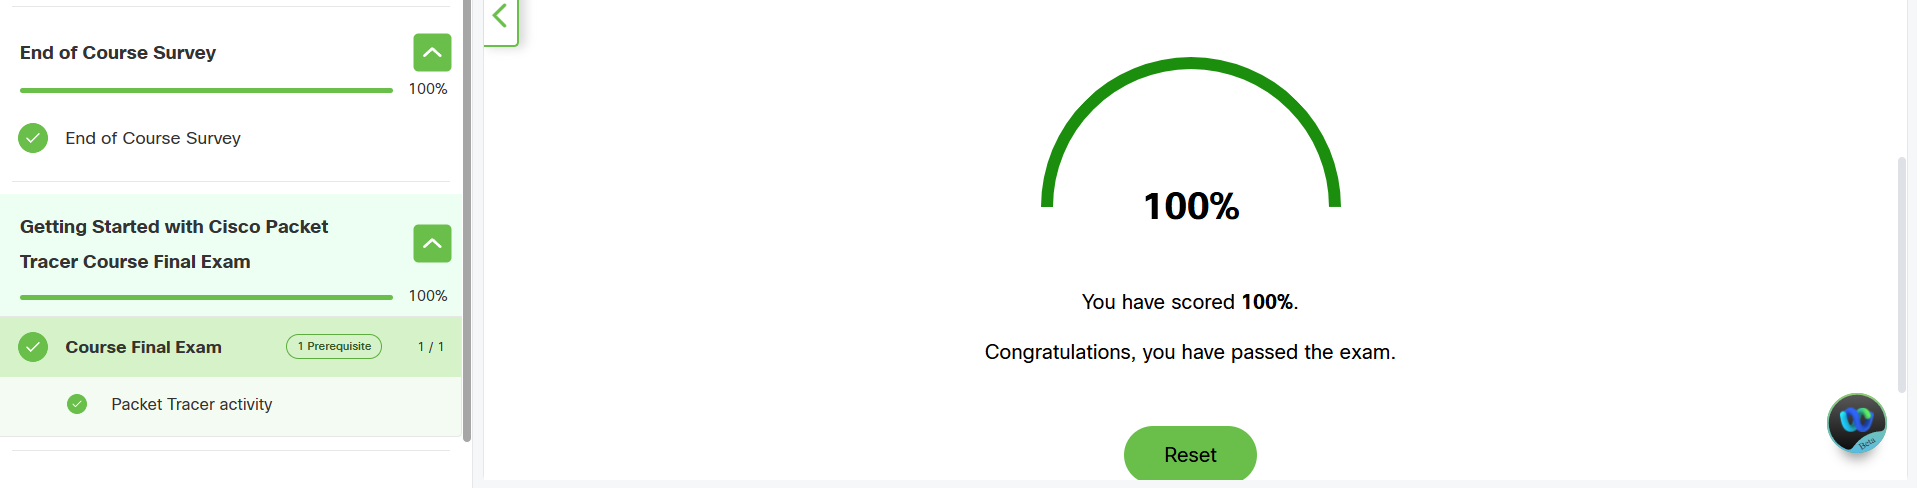
\includegraphics[width=0.7\textwidth]{JuanDavidRangel-ExamGettingStarted.png}
  \caption{Resultado del quiz PT Basics.}
  \label{fig:quiz}
\end{figure}

\textbf{Diagrama de red en Packet Tracer (individual):} topología con 3 routers (Router0 1941, Router1 1841, Router2 1841), switches y servidores, con enlaces Ethernet y un enlace serial entre routers (figura \ref{fig:diagrama}).

\begin{figure}[H]
  \centering
  
\includegraphics[width=0.9\textwidth]{simulacion-de-red.png}
  \caption{Topología de red armada en Packet Tracer.}
  \label{fig:diagrama}
\end{figure}

\textbf{Esquema de direccionamiento aplicado:}
\begin{itemize}
  \item WAN R0--R1: \texttt{7.0.0.0/30} (R0=.1, R1=.2)
  \item WAN R1--R2: \texttt{8.0.0.0/30} (R1=.1, R2=.2)
  \item LAN Router0 VLAN10: \texttt{10.0.10.0/24} (gw 10.0.10.1; Server0 .10, Server1 .11, Switch1 .2)
  \item LAN Router0 VLAN30: \texttt{10.0.30.0/24} (gw 10.0.30.1)
  \item LAN Router2: \texttt{10.0.20.0/24} (gw 10.0.20.1; Server2 .10)
\end{itemize}

\textbf{Respuestas conceptuales:}
\begin{itemize}
  \item \textbf{Conexiones negras sólidas:} enlaces físicos Ethernet directos (cable de cobre) entre dispositivos; la conexión de capa física real que transporta tramas (L1/L2).
  \item \textbf{Conexiones negras punteadas:} conexiones lógicas o virtuales; no hay un cable físico directo, representan una relación lógica entre dispositivos (ruta a través de la red, enlace inalámbrico o un enlace que aún no está activo).
  \item \textbf{Cable serial Router0--Router2:} cable Serial DCE/DTE (rojo) entre los puertos seriales de los routers; el extremo DCE define el clock rate.
\end{itemize}

\subsection{2. Tracking Messages with Packet Tracer}

\textbf{Simulación: ping desde RADIUS hacia DHCP.} Con la topología armada y las IPs configuradas, se activa el modo \emph{Simulation} (abajo a la derecha), se filtran los protocolos \textbf{ICMP} y \textbf{ARP} en \emph{Edit Filters}, y desde la consola del servidor RADIUS se ejecuta un \texttt{ping} a la IP del servidor DHCP.

\textbf{Secuencia de eventos observada:}
\begin{enumerate}
  \item \textbf{ARP Request} (broadcast): RADIUS pregunta ``¿quién tiene la IP del DHCP? Dame tu MAC''.
  \item \textbf{ARP Reply}: el DHCP responde con su MAC.
  \item \textbf{ICMP Echo Request}: mensaje de ping hacia el DHCP.
  \item \textbf{ICMP Echo Reply}: respuesta del DHCP.
\end{enumerate}

Si RADIUS y DHCP están en subredes distintas, entre el ARP y el ICMP aparecen los saltos del router: el paquete viaja con la MAC del siguiente salto en cada enlace, pero la IP origen/destino no cambia (enrutamiento de capa 3).

\textbf{Análisis de las PDUs capa por capa (ICMP Echo Request):}
\begin{itemize}
  \item \textbf{Capa 2 (Ethernet):} MAC origen del RADIUS, MAC destino del DHCP (o del gateway), EtherType \texttt{0x0800} (IPv4).
  \item \textbf{Capa 3 (IP):} IP origen (RADIUS), IP destino (DHCP), protocolo \texttt{1} (ICMP), TTL 128 (decrementa en cada salto de router).
  \item \textbf{Capa 4 (ICMP):} Type \texttt{8} (Echo Request), Code \texttt{0}, con la secuencia del ping.
\end{itemize}

El echo reply es el camino inverso: MACs e IPs intercambiadas y Type \texttt{0} (Echo Reply). El ARP request usa MAC destino \texttt{FF:FF:FF:FF:FF:FF} (broadcast) con EtherType \texttt{0x0806}.

\textbf{Conclusión:} se observa la encapsulación/desencapsulación capa por capa: los datos del ping se encapsulan en un paquete IP y este en una trama Ethernet; en el destino se desencapsula en orden inverso. La IP es la dirección lógica de extremo a extremo (no cambia); la MAC es la dirección física salto a salto (cambia en cada enlace).

\subsection{3. Using Wireshark}

\textbf{¿Qué es Wireshark?} Analizador de protocolos de red (sniffer). Captura paquetes en vivo desde una interfaz, los decodifica capa por capa (Ethernet, IP, TCP/UDP, HTTP, DNS, etc.) y los muestra en tres paneles: lista de paquetes, detalle del paquete y bytes. Es multiplataforma.

\textbf{¿Qué es el modo promiscuo?} Normalmente la NIC solo procesa las tramas dirigidas a su propia MAC (o broadcast/multicast). En modo promiscuo captura TODAS las tramas del medio físico aunque no vayan dirigidas a ella; Wireshark lo usa para ver todo el tráfico del segmento.

\textbf{Captura realizada (16/08/2026, Wireshark 4.6.7):}
\begin{itemize}
  \item Sitio consultado: \texttt{http://www.scielo.org.co} (HTTP en claro, para ver el GET)
  \item Duración: 30 segundos --- Total: 1691 paquetes (1.558.566 bytes)
  \item Peticiones GET capturadas: 4, todas hacia \texttt{168.176.28.57} (servidor de SciELO)
\end{itemize}

\begin{figure}[H]
  \centering
  
\includegraphics[width=0.9\textwidth]{wireshark-captura-scielo.png}
  \caption{Captura en Wireshark del tráfico HTTP hacia scielo.org.co.}
  \label{fig:ws1}
\end{figure}

\textbf{Análisis del paquete GET (frame \#211, 216 bytes) --- encapsulación capa por capa:}

\begin{table}[H]
  \centering
  \begin{tabular}{lll}
    \toprule
    Capa & Protocolo & Datos del paquete \\
    \midrule
    Enlace & Frame Ethernet II & 216 bytes en el cable \\
    Enlace & Ethernet II & MAC destino \texttt{e0:a1:ce:d2:85:76} (router) · MAC origen \texttt{08:f9:7e:9e:25:03} (host) · EtherType IPv4 \\
    Red & IPv4 & Origen \texttt{192.168.1.10} → destino \texttt{168.176.28.57} · TTL 128 \\
    Transporte & TCP & Puerto origen \texttt{60427} (efímero) → puerto \texttt{80} (HTTP) · flags PSH+ACK \\
    Aplicación & HTTP & \texttt{GET / HTTP/1.1} --- petición de la página principal \\
    \bottomrule
  \end{tabular}
  \caption{Desglose del paquete GET analizado.}
\end{table}

\textbf{Observación clave (encapsulación):} cada capa agrega su encabezado a los datos de la capa superior. La petición HTTP va envuelta en TCP (capa 4), luego en IP (capa 3) y luego en Ethernet (capa 2). Al llegar al servidor se desencapsula en orden inverso.

\textbf{Protocolos observados en la captura:}

\begin{table}[H]
  \centering
  \begin{tabular}{lll}
    \toprule
    Protocolo & Paquetes & Nota \\
    \midrule
    QUIC (UDP 443) & 1266 & Tráfico HTTPS moderno de fondo \\
    TCP & 168 & Incluye la conexión HTTP a SciELO \\
    HTTP & 17 & Las 4 peticiones GET + respuestas a SciELO \\
    TLS & 41 & Handshakes HTTPS \\
    DNS & 9 & Resolución de nombres (IPv4 + IPv6) \\
    mDNS & 4 & Descubrimiento local \\
    ICMPv6 & 4 & Vecindario IPv6 \\
    \bottomrule
  \end{tabular}
  \caption{Resumen de protocolos de la captura.}
\end{table}

\begin{figure}[H]
  \centering
  
\includegraphics[width=0.8\textwidth]{red/wireshark-menu.png}
  \caption{Interfaz de Wireshark: menú de captura.}
  \label{fig:ws2}
\end{figure}

\begin{figure}[H]
  \centering
  
\includegraphics[width=0.8\textwidth]{red/wireshark-pantalla-final.png}
  \caption{Pantalla final de Wireshark con el filtro de paquetes HTTP aplicado.}
  \label{fig:ws3}
\end{figure}

\textbf{Videos (evidencia):}
\begin{itemize}
  \item Video 2 --- interfaz y filtros de Wireshark (máx. 5 min; duración 3:37): \href{https://youtu.be/n4p8lmUTW8w}{\url{https://youtu.be/n4p8lmUTW8w}}
  \item Video 3 --- hallazgos de la captura (máx. 7 min; duración 4:29): \href{https://youtu.be/ozmRhLV4BQs}{\url{https://youtu.be/ozmRhLV4BQs}}
\end{itemize}
